\section{Experiments}
\label{sec:exp}

This section presents experimental results using our approach to debug the circuits for a single fix rectification function.
We compare results of our implementation against the incremental SAT-based approach presented in~\cite{fujita:2015}.
The approach presented in~\cite{fujita:2015} is implemented using PICOSAT~\cite{picosat}. The experiments were performed on a 4.0GHz 
Intel(R) $\text{Core}^{\text{TM}}$ i7-6700K Quad-Core CPU with 32 GB of RAM. The data-path sizes {$k$} are selected according to cryptography standards recommended by U.S. National Institute of Standards and Technology (NIST). 
% In our experiments, the labels $NO$, $NM$, and $NI$ denote 
% % the location of unknown component within the circuit topology. Here $NI$, $NM$, and $NO$ 
% that the unknown component is near the input, middle, and near the output, respectively.
We have performed experiments for the cases when the bug is present near 
the input, middle, or near the output, represented using labels $NI$, $NM$, and $NO$ respectively.

\subsection{Word level specification v/s Gate level implementation}
~\autoref{masvsspec} presents the results of our approach with the bug 
in the Mastrovito multiplier and specification is a word level polynomial $f$. 
A Mastrovito multiplier has word level specification $Z = A\times B \pmod{ P(x)}$ 
where $P(x)$ is a given primitive polynomial for the datapath size $k$. The product $A \times B$ 
is computed using an array multiplier architecture, and then the result is reduced modulo $P(x)$. 
The circuit implementation is modeled as a set of polynomials $F=\{f_1,\dots f_i,\dots,f_s\}$. The 
approach then follows the partial reduction of specification polynomial $f$ until leading term of $f_i$ while
recording the intermediate quotients and remainders. We then represent the partial remainder as a linear combination
using the remaining gate polynomials and the quotient, to obtain the solution $P$. We 
are able to verify and debug the circuits for upto 64-bits within our stipulated $TO$ (Time Out) period.

\begin{table}[H]
\centering
\caption{{Single fix rectification debug in Mastrovito circuit against word level specification}. Time is in seconds; $k$ = Datapath Size, \#Gates = No. of gates, K = $10^3$}
\label{masvsspec}
\begin{tabular}{| c | c | c | c | c | c | c | c | c | c | c | c | c | c | c | c | c |} \hline
\multirow{3}{*}{\textbf{k}}& \ #Gates & \multicolumn{15}{ c |}{Our implementation}\\ \cline{3-17}
&&\multicolumn{5}{ c |}{\it NO}&\multicolumn{5}{ c |}{\it NM}&\multicolumn{5}{ c |}{\it NI}\\ \hline
&&{\it a}&{\it b}&{\it c} &{\it d}&{\it e}&{\it a}&{\it b}&{\it c} &{\it d}&{\it e}&{\it a}&{\it b}&{\it c} &{\it d}&{\it e}\\ \hline
9& 0.23K & 0.0 & 0.1 & 0.0 & 0.2 & 0.0 & 0.1 & 0.0 & 0.2 & 0.0 & 0.2 & 0.0 & 0.3\\ \hline
10& 0.29K & 0.0 & 0.3 & 0.0 & 0.3 & 0.0 & 0.3 & 0.0 & 0.3 & 0.0 & 0.4 & 0.0 & 1.4\\ \hline
11& 0.35K & 0.0 & 0.2 & 0.0 & 0.3 & 0.0 & 0.3 & 0.0 & 0.4 & 0.0 & 0.6 & 0.0 & 0.7\\ \hline
12& 0.97K & 0.1 & 7.5 & 0.5 & 8.0 & 0.2 & 10.1 & 0.5 & 10.5 & 0.5 & 121.2 & 0.8 & 121.3\\ \hline
13& 0.82K & 0.1 & 4.3 & 0.3 & 4.5 & 0.2 & 11.3 & 0.6 & 11.2 & 0.7 & 156.3 & 0.8 & 158.1\\ \hline
16& 1.8K & 0.9 & 14.1 & 2.6 & 30.2 & 1.1 & 33.1 & 3.5 & 34.9 & 2.8 & 501.2 & 5.3 & 503.0\\ \hline
32& 5.4K & 36.8 & 378.6 & 110.5 & 544.7 & 40.0 & 567.1 & 160.3 & 767.2 & 38.1 & 1286.1 & 240.3 & 1342.7\\ \hline
%64& 21.8K & 36.8 & 378.6 & 110.5 & 544.7 & 40.0 & 567.1 & 160.3 & 767.2 & 38.1 & 1286.1 & 240.3 & 1342.7\\ \hline
\end{tabular}
\end{table}

Since the SAT-based approach cannot be applied against a word level specification polynomial, 
we perform experiments while using another multiplier implementation as the specification.

% \subsection{Specification and implementation as gate level circuits}

% \subsubsection{Mastrovito v/s Montgomery}
% \begin{figure}[H]
%   \centering
%   %\def\svgwidth{340pt}
%   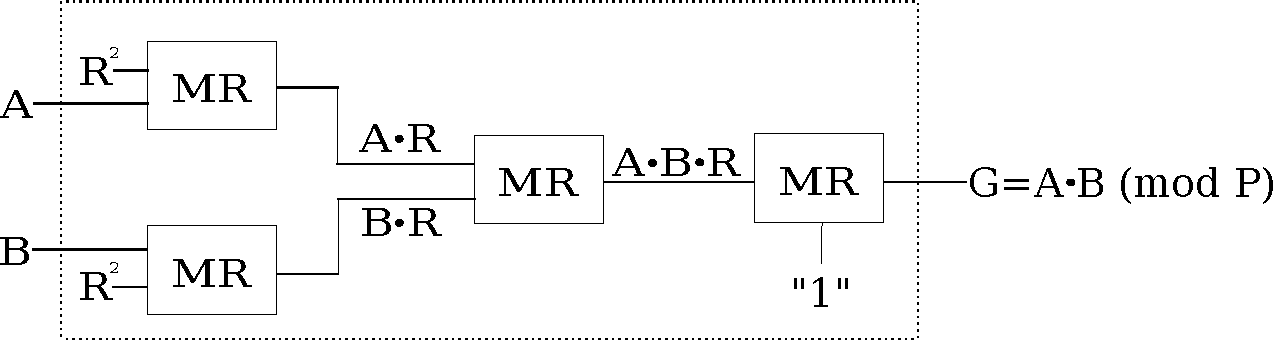
\includegraphics[scale=0.34]{new_mmcircuit-eps-converted-to}
%   \caption{Montgomery multiplication.}
%   \label{montfig}
%   \end{figure}
% Montgomery architectures~\cite{acar:1998},~\cite{wu:2002},
% % \cite{Barrett:1987} 
% ~\cite{knezevic:2008} are considered more efficient than Mastrovito multipliers for exponentiation, 
% as they do not require explicit reduction modulo $P(x)$ after each step.
% ~\autoref{montfig} shows the structure of a Montgomery
% multiplier. Each MR block computes $A\cdot B\cdot R^{-1}$, where $R$
% is selected as a power of a base ($\alpha^{k}$) and $R^{-1}$ is the multiplicative 
% inverse of $R$ in $\mathbb{F}_{2^k}$. As this operation cannot compute $A\cdot B$
% directly, we need to pre-compute $A\cdot R$ and $B\cdot R$ as shown in the~\autoref{montfig}. 
% We denote the leftmost
% two blocks as Block A (upper) and B (lower), the middle block as Block
% C and the output block as Block D.
% % We have presented results for GBR
% %on both \textit{flattened} and \textit{hierarchical} netlists of these
% % multipliers.

% ~\autoref{masusmontspec} presents the results of our approach with an unknown component placed in the Mastrovito multiplier with a Montgomery multiplier circuit used as the specification. While the approach~\cite{fujita:2015} finds a satisfying transformation assignment which can be mapped to a library gate, our approach computes a function which can be implemented as a single gate or sub-circuit. As shown in the table, our approach shows improvement by several orders of magnitude.

% \begin{table}[H]
% \centering
% \caption{{Resolving Unknown Component in Mastrovito circuit with Montgomery circuit as specification}. Time is in seconds; $k$ = Datapath Size, \#Gates = No. of gates, (TO): Time-Out = 3 hrs, K = $10^3$}
% \label{masusmontspec}
% \begin{tabular}{| c | c |  c | c | c | c | c | c |} \hline
% \multirow{3}{*}{\textbf{k}}& \#Gates & \multicolumn{3}{ c |}{Incremental SAT\textbf{~\cite{fujita:2015}}}& \multicolumn{3}{ c |}{Our Approach (\textbf{\autoref{sec:theory}})}\\ \cline{3-8}
% &&{\it NO}&{\it NM}&{\it NI}&{\it NO}&{\it NM}&{\it NI} \\ \hline
% 9& 0.6K &33.7&36.8&34.9& 00.16 & 00.18 & 00.18\\ \hline
% 10& 0.7K &214.3&215&231.4& 00.28 & 00.29 & 00.40\\ \hline
% 11& 0.9K &1,999.5&1,927&2,090.7& 00.49 & 00.49 & 00.63\\ \hline
% 12& 1.6K &24,085&23,400& 8,676& 01.49 & 01.68 & 02.26\\ \hline
% 13& 1.7K & TO&TO&TO& 02.27 & 02.29 & 02.37\\ \hline
% 16& 3K &TO&TO&TO& 13.02 & 15.07 & 26.07\\ \hline
% 32& 9.8K &TO&TO&TO& 1204.03 & 1289.46 & 1870.42\\ \hline
% \end{tabular}
% \end{table}

% % \subsection{Point Addition over Elliptic Curves}
% % Point addition is an important operation required for the task of encryption, decryption 
% % and authentication in Elliptic Curve Cryptography (ECC). 
% % Modern approaches represent the points in projective
% % coordinate systems, {\it e.g.}, the L$\acute{o}$pez-Dahab (LD) projective coordinate, due to which the point addition 
% % operation can be implemented as polynomials in the field. 

% \subsubsection{Agnew's SMPO v/s RH-SMPO}

% The designs discussed so far are combinational implementations of multiplication. 
% These designs use the standard basis representation $\{1,\alpha,\alpha^2, \dots,
% \alpha^{k-1}\}$ to model a $k$-bit data-word $Z$ in terms of its
% constituent bits as $Z = z_0 + z_1 \alpha + z_2 \alpha^2 \cdots +
% z_{k-1} \alpha^{k-1}$, with $\alpha$ being the primitive element for
% that field $\mathbb{F}_{2^k}$. 

% \par 
% %The size of the multipliers presented in the above sections
% %become prohibitively large as $k$ increases.  
% There exists sequential multipliers where $k$-bit inputs are loaded into $k$-bit registers,
% and the $k$-bit result is available  after $k$ clock-cycle execution
% of the machine. These multipliers use a {\it normal basis}
% $\{\beta,\beta^{2},\beta^{4},\dots,\beta^{2^{k-1}}\}$ to  represent a
% $k$-bit data-word $S$ in terms of its constituent bits as $S =
% s_0\beta + s_1\beta^{2} + s_2\beta^{4} \cdots s_{k-1}\beta^{2^{k-1}}$,
% with $\beta$ being the normal element and $\beta=\alpha^m$ for some $m$. 

% We have performed experiments for two types of sequential multipliers namely 
% Agnew's SMPO~\cite{agnew1991implementation} and RH-SMPO~\cite{RHmulti}, where the 
% {\it unknown component} is in the $k$-bit unrolled Agnew's SMPO circuit, and $k$-bit 
% RH-SMPO is used as the specification. The results of this experiment are 
% presented in~\autoref{RHagnew}.

% \begin{table}[H]
% \centering
% \caption{{Resolving Unknown Component in Agnew's SMPO circuit against RH-SMPO circuit implementation}. Time is in seconds; $k$ = Datapath Size, \#Gates = No. of gates, K = $10^3$}
% \label{RHagnew}
% \begin{tabular}{| c | c | c | c | c |} \hline
% \multirow{2}{*}{\textbf{k}}& \#Gates & \multicolumn{3}{ c |}{Our implementation~(\autoref{sec:theory})}\\ \cline{3-5}
% &&{\it NO}&{\it NM}&{\it NI}\\ \hline
% 18& 2K &01.60 & 01.63 & 01.82\\ \hline
% 33& 6.7K &97.14 & 100.03 & 102\\ \hline
% 51& 16K &1320 & 1356 & 1410\\ \hline
% \end{tabular}
% \end{table}

% We are working on further improving the experiments by employing better data structures like
% ZBDDs~(\cite{minato:zbdd}), and devising better heuristics to represent the
% partial remainder as a linear combination of an ideal.